\chapter{Analýza}

\indent

Poněvadž původní záměr zněl rozšířit mobilní aplikaci Catcher,
měli bychom se v této kapitole zabývat jejím průzkumem. Neopomene ani jiné podobné projekty.
V druhé části se podíváme na možnosti našeho řešení.

\section{Existující řešení}

\subsection*{Mobilní aplikace Catcher}

\indent

V roce 2013 \cite{cald-catcher} byla zveřejněna první verze této aplikace pro mobilní telefony s operačním systémem Android.
Autory byli dva aktivní hráči Jiří Voseček a Ondřej Burkert. Aplikace si dobu od svého vzniku získala velkou popularitu
ve~frisbee komunitě a dnes je používaná na většině českých turnajů. Umí zadávat výsledky
zápasů včetně podrobného průběhu bodů, rozhodovat o umístění v základních skupinách, počítat statistiky hráčů napříč
všemi zápasy na turnaji, odevzdávat a zveřejnit vzájemná hodnocení SOTG týmů na turnaji. Dokáže omezeně importovat oficiální soupisky týmů
na nadcházející turnaje spadající pod Českou asociaci létajícího talíře.

\medskip

Kromě mobilní aplikace Catcher byl vytvořen backend v PHP, který ukládá a počítá data na serveru. Ten nicméně není
objektově orientovaný a všechna jeho eventuální rozšíření jsou velmi náročná.

\subsubsection*{Výhody}
\begin{itemize}
  \item Všechny výsledky se přehledně zobrazují na webu frisbee.cz.
  \item Existuje fungující aplikace na OS Android.
  \item Přes webový prohlížeč lze přistupovat k emulátoru aplikace.
  \item Systém je již mezi organizátory turnajů zaběhnutý a na Google Play
    \footnote{Online distribuční služba, kde jsou k dispozici aplikace pro mobilní telefony a tablety s OS Android}
    má již více než 1000 stáhnutí \cite{catcher-play}.
\end{itemize}

\begin{figure}[ht!]
\centering

\includegraphics[width=60mm]{./images/catcher.png}
\caption{Mobilní aplikace Catcher \cite{catcher-play}.\label{overflow}}
\label{fig:uwsgi}
\end{figure}

\subsubsection*{Nevýhody}
\begin{itemize}
  \item Import soupisek z databáze ČALD je pouze poloautomatický. Některý z adminů musí před každým turnajem
    import spustit a zkontrolovat, zda se data uložily validně. Tomuto stavu nepřispívá ani fakt,
    že databáze ČALD, ze které se import provádí, je velmi špatně navržena a v nejbližších měsících čeká na svoji novou verzi.
  \item Nedisponuje žádným efektivním webovým rozhraním.
  \item Automaticky nedoplňuje týmy v zápasech play-off do dalších kol (např. vítěze semifinále do finále apod.).
  \item Při vytváření turnaje neprobíhá žádná kontrola validity dat.
    Lze tak vytvořit spoustu chybných utkání, které pak musí administrátor manuálně mazat z databáze. 
\end{itemize}

\subsection*{Ultimate Organizer}

Aplikace zveřejněná v roce 2004 \cite{ultimate-organizer}, napsaná v PHP a používaná na velkých akcích jako mistrovství světa nebo Evropy
pro sledování výsledků a statistik. Poskytuje tvorbu a správu turnajů, týmů, hráčů,
výsledků, rozpisů atd. Podporuje vícejazyčnost, tisk rozpisů v PDF, přístup pro mobilní telefony
a~spoustu dalších vlastností. Dokáže zobrazit podrobné detaily o průběhu zápasů.

\subsubsection*{Výhody}
\begin{itemize}
  \item Rozsáhlá aplikace poskytující nepřeberné množství možností.
  \item Aplikace již má za sebou více než 10 let fungování.
  \item Poskytuje přístup pro mobilní telefony s webovým prohlížečem.
\end{itemize}

\subsubsection*{Nevýhody}
\begin{itemize}
  \item Aplikace nefunguje jako webová služba. Uživatel si musí stáhnout zdrojové kódy a aplikaci si sám nasadit na svém počítači nebo serveru.
  \item Neposkytuje žádné rozumné rozhraní, tudíž pro ni nelze vytvořit žádného klienta.
  \item Nelze sledovat dlouhodobější statistiky napříč týmy a hráči. Všechny výsledky se týkají pouze jednoho konkrétního turnaje.
\end{itemize}

\subsection*{Ultimate Central}

Webová služba, která spíš než ke statistikám slouží k správě soupisek na turnajích. Pořadatel turnaje vytvoří událost
v kalendáři a zapíše všechny účastnící se týmy. Ty pak musí odevzdat svoje soupisky a potvrdit náležité dokumenty,
které se na některých turnajích stávají povinností (např. zřeknutí se možnosti žalovat organizátora aj.).

\begin{figure}[ht!]
\centering
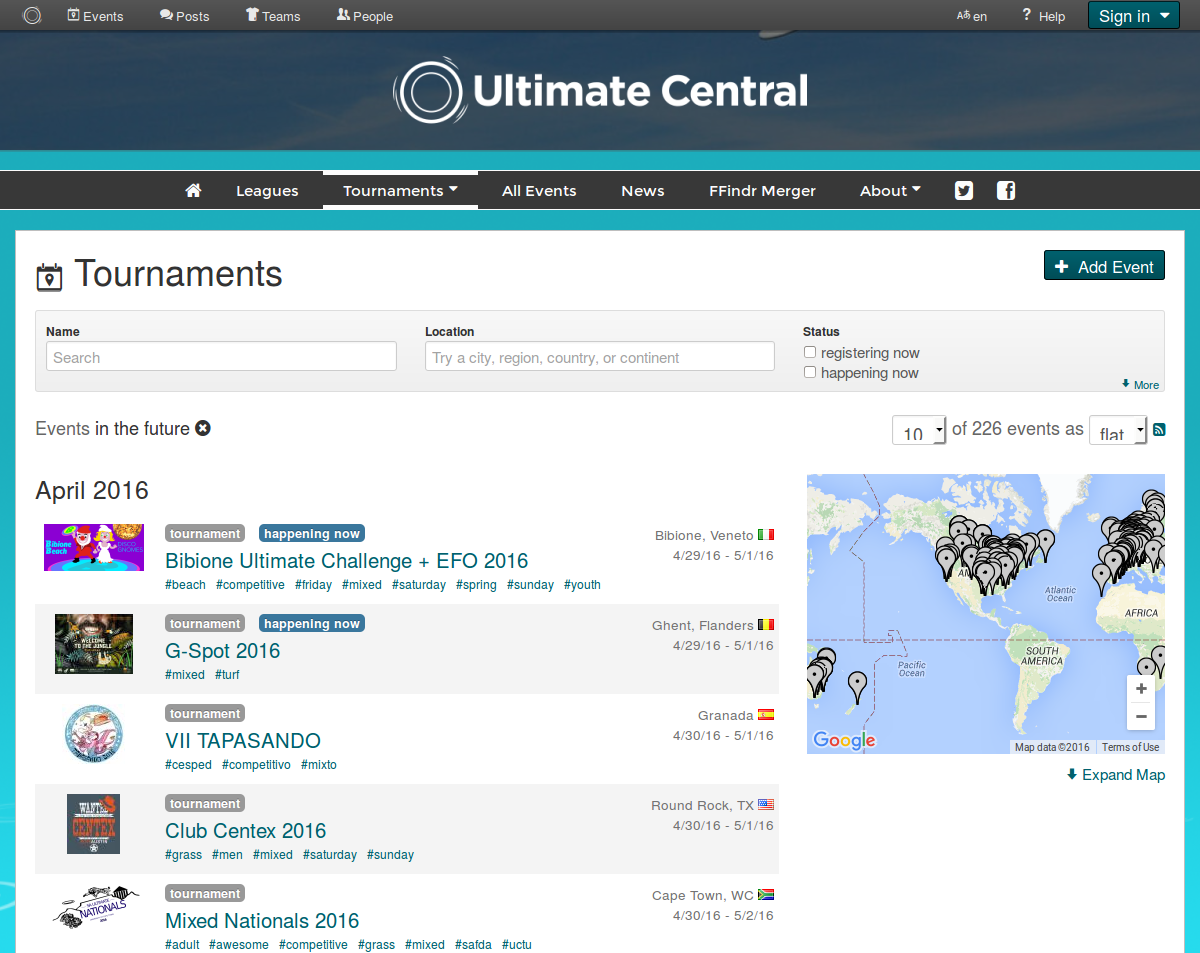
\includegraphics[width=130mm]{./images/ultimate-central.png}
\caption{Webová aplikace Ultimate Central.\label{overflow}}
\label{fig:uwsgi}
\end{figure}

\subsubsection*{Výhody}
\begin{itemize}
  \item Umožňuje vytvořit jednoduchou webovou stránku pro každý turnaj, na které lze shrnout důležité informace pro všechny účastníky.
  \item Aplikace je dostupná ve webovém prohlížeči.
\end{itemize}

\subsubsection*{Nevýhody}
\begin{itemize}
  \item Neslouží ke statistikám. Do systému se zapisují pouze výsledky a hodnocení SOTG.
  \item Vyžaduje registraci a přihlašení každého jednotlivého hráče na turnaji.
  \item Stejně jako obě předchozí aplikace neposkytuje rozhraní, které by mohla využít například mobilní aplikace.
\end{itemize}

\subsection{Výsledek}

\indent

Průzkum existujících řešení naznačil, že náš projekt má smysl. Stále chybí aplikace,
která by byla plně automatizovaná (před započetím turnaje se vytvoří rozpis a~ten se
již doplňuje na základě zadaných výsledků), měla rozhraní pro libovolné tenké klienty
a~dokázala použít data z~databáze ČALD.

\section{Možnosti řešení}

\indent

Protože už od počátku známe požadavek na možnost připojení klienta v~podobě mobilní nebo jiné webové aplikace,
je nutné poskytnout žadatelům o~přístup k datům rozhraní, které dostatečně pokryje jejich požadavky.
V našem případě je symbolizují již výše zmíněné případy užití.

% TODO: jestli by nebylo lepsi tuhle cast presunout do uvodu do probelmatiky?

\textit{Nějaký kecy o tom, jak mám možnost použít SOAP a REST z úvodní kapitoly.}

\subsubsection*{SOAP}

\indent

Protokol SOAP (\textit{Simple Object Access Protocol}) vystavuje aplikační logiku jako službu
a~je proveden v~syntaxi jazyka XML. Svým navržením se snaží
být co nejméně závislý na zvolené verzi standartu XML.
SOAP služby standartně obsahují v URL nějaké sloveso (např. zobrazInfo).
